\documentclass[UKenglish]{beamer}


\usetheme{UiB}


\usepackage[utf8]{inputenx} % For æ, ø, å
\usepackage{csquotes}       % Quotation marks
\usepackage{microtype}      % Improved typography
\usepackage{amssymb}        % Mathematical symbols
\usepackage{mathtools}      % Mathematical symbols
\usepackage[absolute, overlay]{textpos} % Arbitrary placement
\setlength{\TPHorizModule}{\paperwidth} % Textpos units
\setlength{\TPVertModule}{\paperheight} % Textpos units
\usepackage{tikz}
\usepackage{minted}
\usetikzlibrary{overlay-beamer-styles}  % Overlay effects for TikZ


\author{Cauchy Pu}
\title{Assembly}
\subtitle{Where we stand and where we go}


\begin{document}


% Use
%
%     \begin{frame}[allowframebreaks]{Title}
%
% if the TOC does not fit one frame.

\begin{frame}
\frametitle{Outline}
\tableofcontents
\end{frame}

\section{Overview}
\begin{frame}{Overview}
  Computers execute machine code, sequences of bytes encoding the low-level operations
  that manipulate data, manage memory, read and write data on storage devices, and
  communicate over networks.

  \begin{alertblock}{Bits and Where}
   Information = Bits + Context
 \end{alertblock}

 \begin{center}
   \structure{So we study what bits and in which we view them}\\ \\
 \end{center}

 \begin{center}
   \vspace{1cm}
   \Huge Assembly!
 \end{center}
\end{frame}


\section{Why assembly}
\begin{frame}{Why assembly}
  But, compilers do most of the work in generating assembly code, so why sould we spend
  our time?
  \begin{enumerate}
  \item Optimization. Sometimes we have to try the assembly code corresponding to various
    forms of upper language.
  \item Some bugs more obvious in assembly. For exmaple, concurrent programs.
  \item Security. Overwrite information is a common attack method.
  \item Some code must be assembly, context switch.
  \item When you encounter core dump, what the corresponding high level code?
  \item And you told me, we are low-level engineer, right? So, here we go, assembly!
  \item ......
  \end{enumerate}
   \begin{center}
   \Huge Think like a computer
 \end{center}
\end{frame}

\begin{frame}{Why assembly}
  \begin{example}
    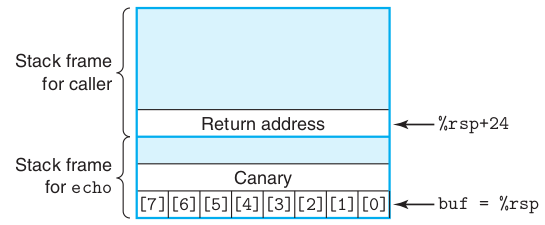
\includegraphics[width = \textwidth, height=2cm]{canary.png}
    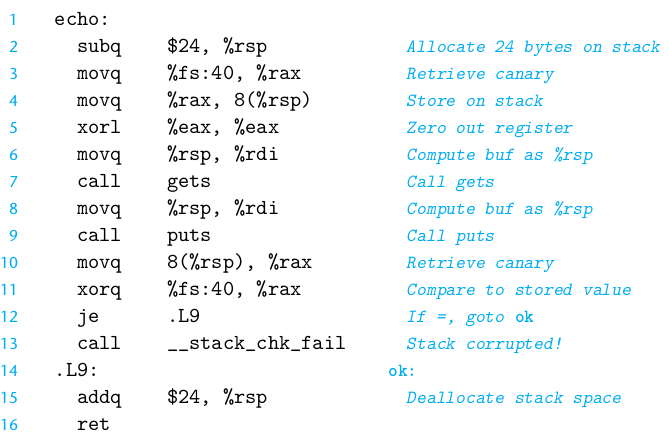
\includegraphics[width = \textwidth, height=4.5cm]{canary_assembly.png}
  \end{example}
\end{frame}

%high language how to map to assembly, instructions
\section{A simple world}
\begin{frame}{A simple world}
  In the world of assembly...
  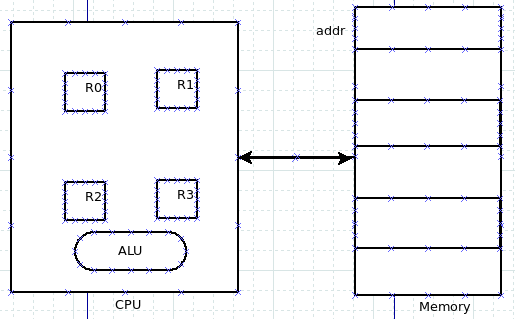
\includegraphics[width = \textwidth, height=4.5cm]{simple.png}
  \begin{center}
   \Huge Simple, right?
  \end{center}
\end{frame}

\begin{frame}{A simple world}
  The class of instructions:
  \begin{enumerate}
  \item assessing
    \begin{itemize}
    \item mov
    \item ldl
    \item stl
    \end{itemize}
  \item arithmetic and logical operations
    \begin{itemize}
  \item add
  \item sub
    \end{itemize}
  \item control \& procedures
    \begin{itemize}
  \item jump
  \item call
  \item ret
    \end{itemize}
  \end{enumerate}
\end{frame}

\begin{frame}{A simple world}
  How stack operations...
  \begin{center}
    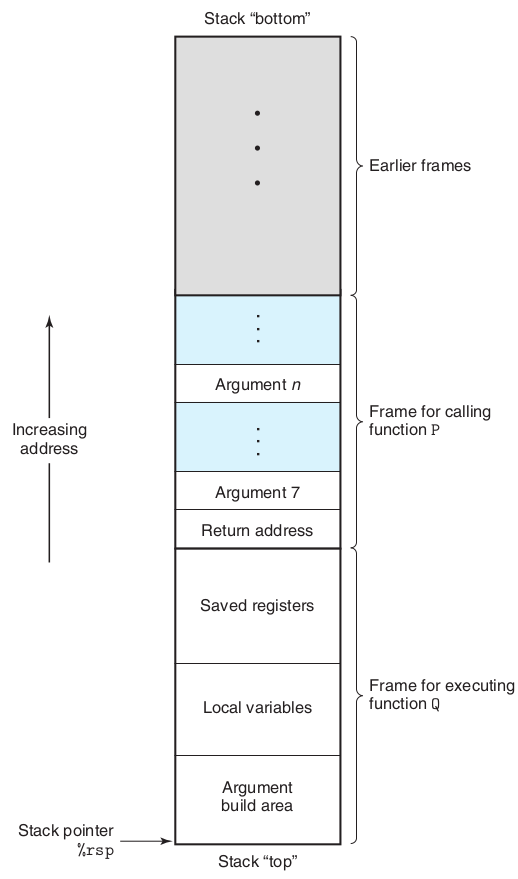
\includegraphics[width = 0.8\textwidth, height=7.5cm]{stack.png}
  \end{center}
\end{frame}

\section{Inline Assembly}
\begin{frame}{Inline Assembly}
  When you travel happily in the kernel source...
  \begin{alertblock}{Damn!}
\begin{verbatim*}
__asm__ __volatile__(
    "movl %6,%%edi\n\t"
    "repne\n\t"
    "scasb\n\t"
    "notl %%ecx\n\t"
    "decl %%ecx\n\t"    /* NOTE! This also sets Z if searchstring='' */
    "movl %%ecx,%%edx\n"
    "1:\tmovl %6,%%edi\n\t"
    "movl %%esi,%%eax\n\t"
    "movl %%edx,%%ecx\n\t"
    "repe\n\t"
    "cmpsb\n\t"
    "je 2f\n\t"     /* also works for empty string, see above */
    "xchgl %%eax,%%esi\n\t"
    "incl %%esi\n\t"
    "cmpb $0,-1(%%eax)\n\t"
    "jne 1b\n\t"
    "xorl %%eax,%%eax\n\t"
    "2:"
    : "=a" (__res), "=&c" (d0), "=&S" (d1)
    : "0" (0), "1" (0xffffffff), "2" (cs), "g" (ct)
    : "dx", "di");
return __res;
\end{verbatim*}
 \end{alertblock}
  
\end{frame}

\section{How many architectures}
\begin{frame}{How many architectures}
  
\end{frame}

% abi
\section{Agreements}
\begin{frame}{Agreements}
  
\end{frame}

\section{Reverse Engineering}
\begin{frame}{Reverse Engineering}
  
\end{frame}

\section{References}
\begin{frame}[allowframebreaks]{References}
    \begin{thebibliography}{}

        % Article is the default.
        \setbeamertemplate{bibliography item}[book]
        \bibitem{Hartshorne1977}
         Randal E. Bryant, David R. O'Hallaron
        \newblock \emph{Computer Systems, A prorgammer's perspective}.
        \newblock Pearson, 2018
        \end{thebibliography}
\end{frame}


\end{document}